%!TEX root = ../thesis.tex
%*******************************************************************************
%****************************** Second Chapter *********************************
%*******************************************************************************
\chapter{Literature Review} \label{sec:Literature Review}

\graphicspath{{Chapter2/Figs/}}
This chapter lays down the fundamental theories of optoelectronics and search algorithms, which are essential to the research outlined in the later chapters of this thesis.

\section{Fourier Optics}

\subsection{The Propagation of Light}
\subsubsection{Wave-Particle Duality}
The problem of how light propagates has been troubling scientists for centuries. The journey began with Sir Isaac Newton, who advocated the particle theory of light in the 17th century. Newton proposed that light consists of particles, or `corpuscles', which explained phenomena such as reflection and refraction \cite{Newton1704}. In contrast, Christiaan Huygens, a contemporary of Newton, demonstrated that light behaves as a wave, as it is capable of diffraction and interference \cite{Huygens1690}.

\begin{figure}[H]
	\centering
	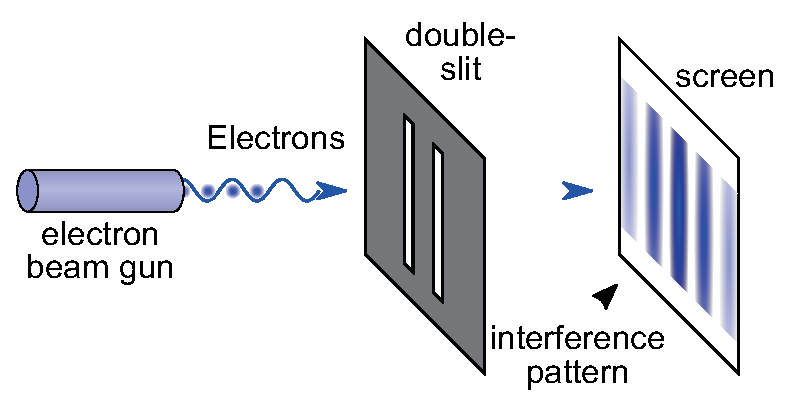
\includegraphics[width=0.7\textwidth]{Double-slit.eps}
	\caption{An illustration of the Young's Double-slit experiment \cite{Kalliauer2017}}
	\label{fig:Double-slit.eps}
\end{figure}

The wave theory gained significant support in the early 19th century through the experiments of Thomas Young. Young's double-slit experiment in 1801 provided clear evidence of the wave nature of light by showing that light passing through two slits creates an interference pattern on a screen \cite{Young1802}, as illustrated in \cref{fig:Double-slit.eps}. Augustin-Jean Fresnel further advanced the wave theory by developing a comprehensive mathematical framework to describe light as a wave, explaining phenomena such as polarization and the diffraction of light \cite{Fresnel1826}.

This understanding was further reinforced by James Clerk Maxwell in the mid-19th century. In 1864, James Clerk Maxwell organised a set of four equations describing the space and time dependence of the electromagnetic field, which are:
\begin{align}
  \nabla \times \mathbb{E} & = -\frac{\partial \mathbb{B}}{\partial t}             \label{eq:maxwell1} \\
  \nabla \times \mathbb{H} & = \mathbb{J} + \frac{\partial \mathbb{D}}{\partial t} \label{eq:maxwell2} \\
  \nabla \cdot \mathbb{D}  & = \rho                                                \label{eq:maxwell3} \\
  \nabla \cdot \mathbb{B}  & = 0 \label{eq:maxwell4}
\end{align}
where $\mathbb{D}$ is the electric flux density, $\mathbb{E}$ is the electric field intensity, $\mathbb{B}$ is the magnetic flux density, $\mathbb{H}$ is the magnetic field intensity, $\rho$ is the volume charge density, and $\mathbb{J}$ is the current density \cite{Daintith2009}.

And the relation between $\mathbb{D}$ and $\mathbb{E}$ and between $\mathbb{B}$ and $\mathbb{H}$ for linear materials are:
\begin{align}
  \mathbb{B} & = \mu \mathbb{H}      \\
  \mathbb{D} & = \epsilon \mathbb{E}
\end{align}
where $\mu$ is the magnetic permeability and $\epsilon$ is the dielectric permittivity of the material \cite{Wilkinson2017}.

Maxwell's equations unified electricity and magnetism into a single theory of electromagnetism, predicting that light is an electromagnetic wave that propagates through space \cite{Maxwell1865}.

Despite the success of the wave theory, it could not explain all light-related phenomena. The early 20th century brought a pivotal development with Albert Einstein's explanation of the photoelectric effect. In 1905, Einstein proposed that light also behaves as particles, or `quanta' (later called photons), which could eject electrons from a metal surface when light is shone upon it \cite{Einstein1905}. This particle nature of light was critical in explaining observations that wave theory alone could not address and earned Einstein the Nobel Prize in Physics in 1921.

These discoveries collectively revealed that light exhibits both wave and particle properties, depending on the experimental context. This wave-particle duality became a cornerstone of quantum mechanics, fundamentally altering human's understanding of the nature of light. Although to date, it is still not yet known what light exactly is, it is now known how light behaves.

\subsubsection{Wave Equation}
To mathematically describe the propagation of light in free space (i.e. in absence of free charge), the Maxwell equations in \cref{eq:maxwell1} - \cref{eq:maxwell4} can be simplified as:
\begin{align}
  \nabla \times \mathbb{E}         & = -\mu \frac{\partial \mathbb{H}}{\partial t}     \label{eq:simplified_maxwell1} \\
  \nabla \times \mathbb{H}         & = \epsilon \frac{\partial \mathbb{E}}{\partial t} \label{eq:simplified_maxwell2} \\
  \nabla \cdot \epsilon \mathbb{E} & = 0                                               \label{eq:simplified_maxwell3} \\
  \nabla \cdot \mu \mathbb{H}      & = 0 \label{eq:simplified_maxwell4}
\end{align}

Taking the curl on both the left and right hand sides of \cref{eq:simplified_maxwell1}, and using the vector identity of $\nabla \times (\nabla \times \textbf{u}) = \nabla(\nabla \cdot \textbf{u}) - \nabla^2 \textbf{u}$, we get:
\begin{align}
  \nabla \times (\nabla \times \mathbb{E})               & = -\nabla \times (\mu \frac{\partial \mathbb{H}}{\partial t}) \label{eq:wave_equation_derivation1} \\
  \nabla (\nabla \cdot \mathbb{E}) - \nabla^2 \mathbb{E} & = -\frac{\partial}{\partial t} \nabla \times (\mu \mathbb{H}) \label{eq:wave_equation_derivation2}
\end{align}

Then, by substituting \cref{eq:simplified_maxwell2} and \cref{eq:simplified_maxwell3} in, \cref{eq:wave_equation_derivation2} becomes:
\begin{equation}
  -\nabla^2 \mathbb{E} = -\frac{\partial}{\partial t} (\mu \epsilon \frac{\partial \mathbb{E}}{\partial t}) \label{eq:wave_equation_derivation3}
\end{equation}

Hence, we have a generic form of wave equation, relating the space and time domain relation of electromagnetic waves propagating in free space:
\begin{equation}
  \nabla^2 \mathbb{E} = \mu \epsilon \frac{\partial^2 \mathbb{E}}{\partial t^2} \label{eq:wave_equation}
\end{equation}

A valid solution to \cref{eq:wave_equation} is:
\begin{equation}
  \mathbb{E} = \mathbb{E}_0 e^{j(\omega t - k r)} \label{eq:wave_equation_solution}
\end{equation}
where $\omega$ is the angular velocity of the wave, $t$ is time, $r$ is the propagation distance and $k$ is called the wave number ($k=\frac{2\pi}{\lambda}$, where $\lambda$ is the wavelength). From \cref{eq:wave_equation_solution} we can see that the propagation of light in free space is essentially a phase shift. This suggests that, if we have a coherent light source and a device to manipulate light (called spatial light modulator, further explained in \cref{sec:SLM}), we can produce an interference pattern reconstructing the target field we desire, and such method is called holographic projection.



\subsection{Diffraction} \label{sec:Diffraction}

\subsubsection{Diffraction Through a Two-Dimensional (2D) Aperture}
\begin{figure}[H]
  \centering
  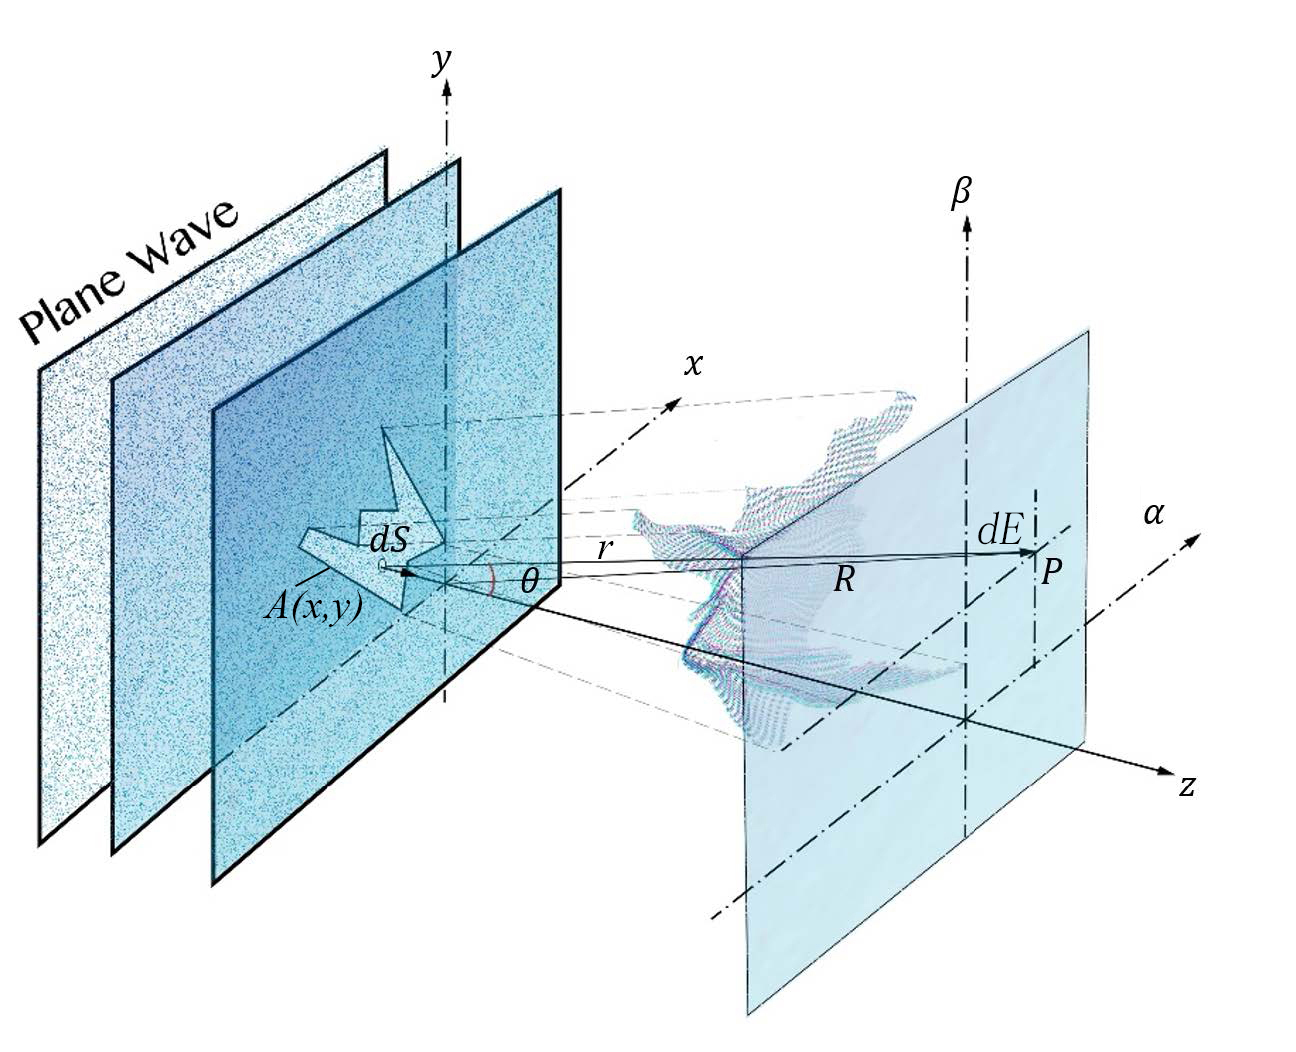
\includegraphics[width=0.7\textwidth]{diffraction_coordinate_definition.jpg}
  \caption{Diffraction geometry}\label{fig:diffraction_coordinate_definition}
\end{figure}

To model how light diffracts through a 2D aperture, we first set up a coordinate system as shown in \cref{fig:diffraction_coordinate_definition}, where the aperture is denoted by $A(x, y)$ and the diffracted field is denoted by $E(\alpha, \beta, z)$.

\begin{figure}[H]
  \centering
  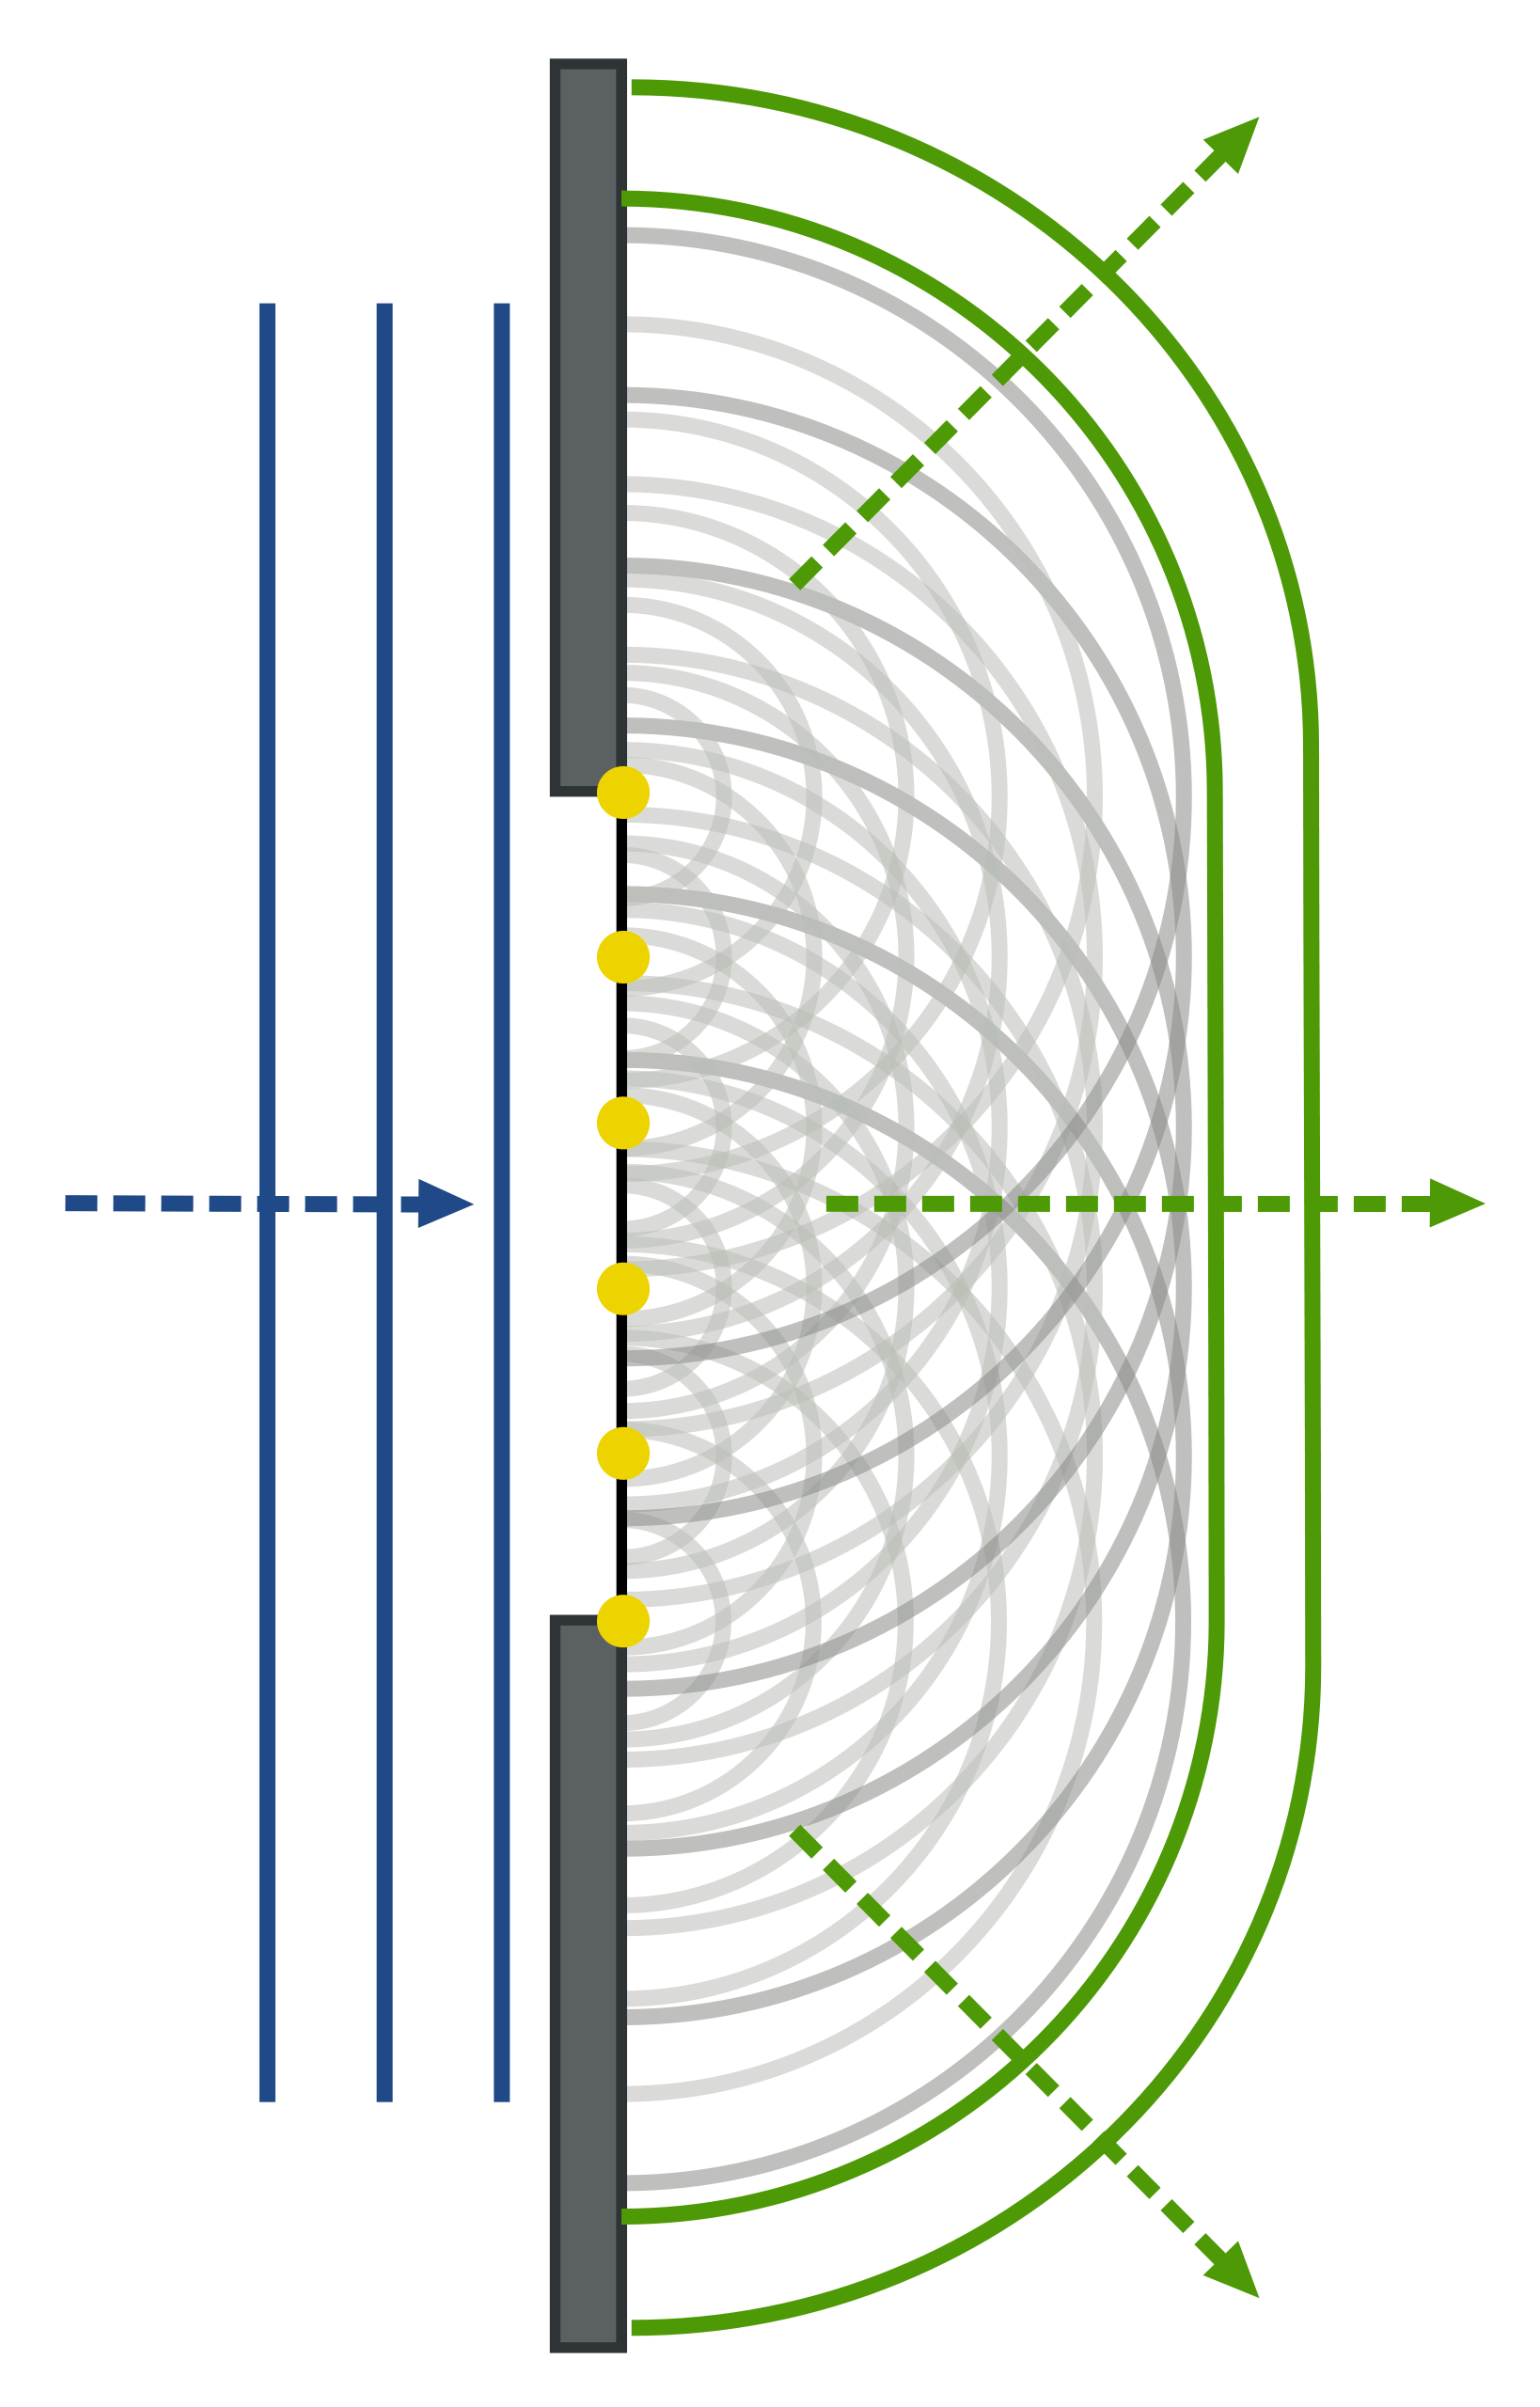
\includegraphics[width=0.2\textwidth]{huygens_wavelets_principle.png}
  \caption{Huygens-Fresnel wavelet principle \cite{Nordmann2007}}\label{fig:huygens_wavelets_principle}
\end{figure}

Huygens-Fresnel principle states that every point on a wavefront is itself the source of outgoing secondary spherical wavelets, which can be expressed mathematically as follows when $r\gg \lambda$ \cite{Goodman2017}:
\begin{equation}
  E(\alpha, \beta, z) = \frac{1}{j\lambda} \iint A(x,y)\frac{e^{jkr}}{r} cos(\theta) dxdy \label{eq:huygens-fresnel-principle}
\end{equation}

And by trigonometry we can have the following identities:
\begin{align}
  cos(\theta) & = \frac{z}{r}                                               \\
  R^2         & = \alpha ^2 + \beta ^2 + z^2       \label{eq:trignometry-R} \\
  r^2         & = (\alpha-x)^2 + (\beta-y)^2 + z^2 \label{eq:trignometry-r}
\end{align}

Then \cref{eq:huygens-fresnel-principle} becomes:
\begin{align}
  E(\alpha, \beta, z) & = \frac{z}{j\lambda} \iint A(x,y)\frac{e^{jkr}}{r^2} dxdy                    \label{eq:huygens-fresnel-principle-substituded-cos}                                                      \\
                      & = \frac{z}{j\lambda} \iint A(x,y)\frac{e^{jk\sqrt{(\alpha-x)^2 + (\beta-y)^2 + z^2}}}{(\alpha-x)^2 + (\beta-y)^2 + z^2} dxdy \label{eq:huygens-fresnel-principle-substituded-r-square}
\end{align}

Unfortunately, \cref{eq:huygens-fresnel-principle-substituded-r-square} can only be solved analytically for few specific aperture functions $A(x,y)$, so we have to make some approximations to solve for arbitrary $A(x,y)$, the common methods are \textit{Fresnel} and \textit{Fraunhofer} approximations for regions depicted in \cref{fig:fresnel_fraunhofer_approximations} below.

\begin{figure}[H]
  \centering
  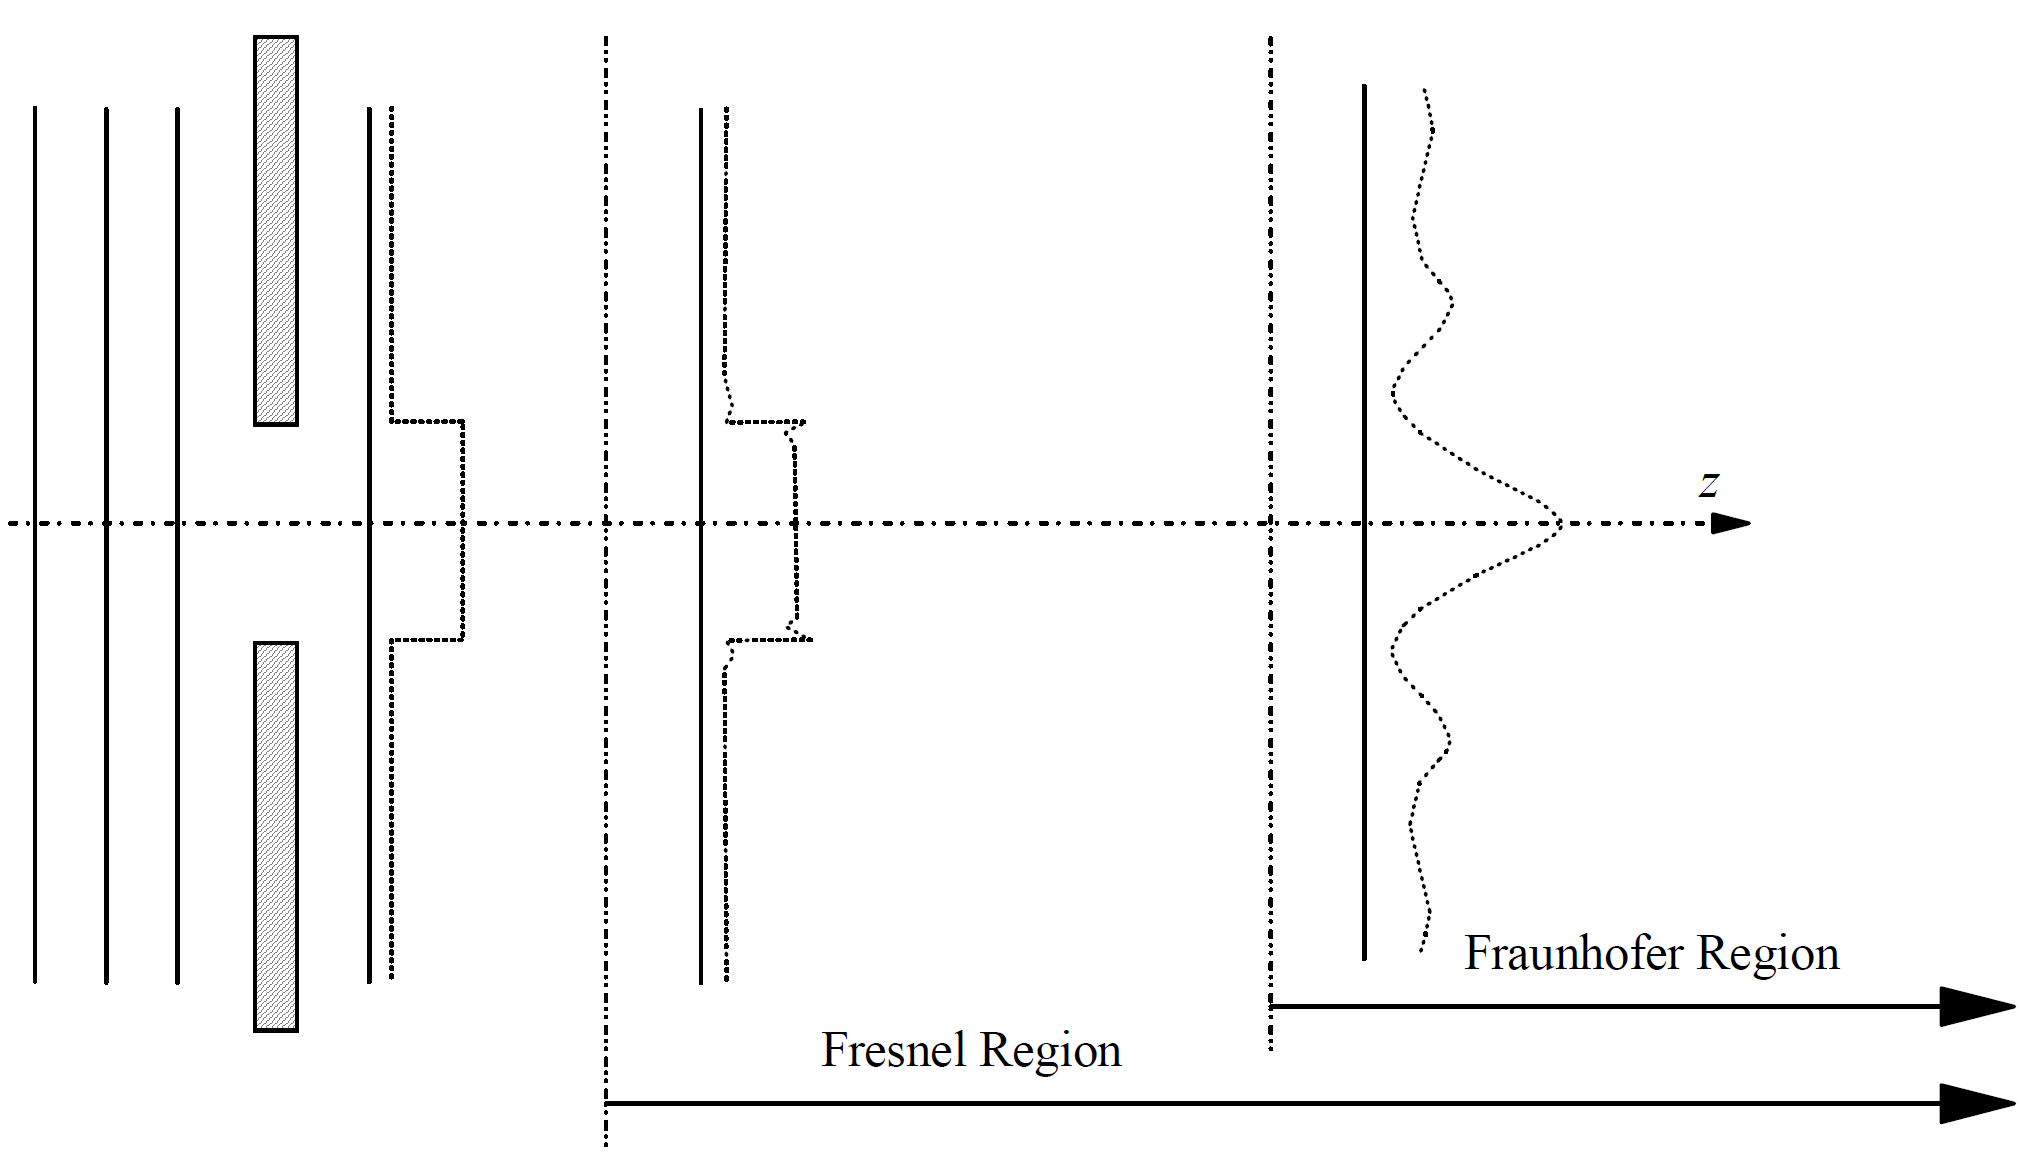
\includegraphics[width=0.7\textwidth]{fresnel_fraunhofer_approximations.png}
  \caption{Fresnel and Fraunhofer region \cite{Wilkinson2019}}\label{fig:fresnel_fraunhofer_approximations}
\end{figure}


\subsubsection{Fresnel Approximation}

Fesnel approximation replaces expressions for spherical waves by quadratic-phase exponentials, using the binomial expansion of the square root to approximate $r$ in \cref{eq:huygens-fresnel-principle-substituded-cos} \cite{Goodman2017}:
\begin{equation}
  \sqrt{1+d} = 1 + \frac{1}{2}d - \frac{1}{8}d^2 + \cdots \label{eq:binomial-expension}
\end{equation}

Retaining only the first two terms of the expansion in \cref{eq:binomial-expension}, and substituting in \cref{eq:trignometry-r} gives:
\begin{align}
  r & = \sqrt{(\alpha-x)^2 + (\beta-y)^2 + z^2}                                                                                                              \\
    & = z \sqrt{1 + \left( \frac{\alpha-x}{z} \right)^2 + \left(\frac{\beta-y}{z}\right)^2}                                                                  \\
    & \approx z \left[ 1 + \frac{1}{2} \left( \frac{\alpha-x}{z} \right)^2 + \frac{1}{2} \left(\frac{\beta-y}{z}\right)^2 \right] \label{eq:r-approximation}
\end{align}

For the $r^2$ in the denominator of \cref{eq:huygens-fresnel-principle-substituded-cos}, the error introduced by dropping all terms but $z$ is generally acceptably small, but for the $r$ appearing in the exponent in the numerator of \cref{eq:huygens-fresnel-principle-substituded-cos}, errors are much more critical \cite{Goodman2017}. So, by substituting \cref{eq:r-approximation} for the $r$ in the numerator of \cref{eq:huygens-fresnel-principle-substituded-cos} and substituting $z$ for the $r$ in the denominator, we have:
\begin{align}
  E(\alpha, \beta, z) & = \frac{z}{j\lambda} \iint A(x,y)\frac{e^{jkz \left[ 1 + \frac{1}{2} \left( \frac{\alpha-x}{z} \right)^2 + \frac{1}{2} \left(\frac{\beta-y}{z}\right)^2 \right]}}{z^2} dxdy \\
                      & = \frac{e^{jkz}}{j\lambda z} e^{j\frac{k}{2z}(\alpha^2+\beta^2)} \iint \left\{A(x,y)e^{j\frac{k}{2z}(x^2+y^2)}\right\}e^{-j\frac{2\pi}{\lambda z}(\alpha x+\beta y)}dxdy    \\
                      & = \frac{e^{jkz}}{j\lambda z} e^{j\frac{k}{2z}(\alpha^2+\beta^2)} \mathcal{F} \left\{A(x,y)e^{j\frac{k}{2z}(x^2+y^2)}\right\}
\end{align}
where $\mathcal{F}$ is the Fourier Transform.

Now we have a more simple and solvable expression than \cref{eq:huygens-fresnel-principle-substituded-r-square}. And also, as we are only interested in the scaling of relative points at $P$ with respect to each other, so it is safe to normalise the multiplier term before the Fourier Transform to 1 \cite{Wilkinson2019}. So we can express the diffraction pattern in Fresnel region as:
\begin{equation}
  E_{Fresnel\ region}(\alpha, \beta, z) = \mathcal{F} \left\{A(x,y)e^{j\frac{k}{2z}(x^2+y^2)}\right\} \label{eq:fresnel-diffraction}
\end{equation}


\subsubsection{Fraunhofer Approximation}
Fraunhofer diffraction is a form of diffraction in which the distance between the light source and the receiving screen are in effect at infinite, so that the wave fronts can be treated as planar rather than spherical \cite{Daintith2009}. Fraunhofer approximation is very stringent, it assumes that the distance between the light source and the receiving screen are in effect at infinite:
\begin{equation}
  z\gg \frac{k(x^2+y^2)_{max}}{2}
\end{equation}

so that the wave fronts can be treated as planar rather than spherical \cite{Daintith2009}, then the $e^{j\frac{k}{2z}(x^2+y^2)}$ term tends to $1$, and \cref{eq:fresnel-diffraction} becomes:
\begin{equation}
  E_{Fraunhofer\ region}(\alpha, \beta) = \mathcal{F} \left\{A(x,y)\right\}
\end{equation}

which suggests that the far field pattern is simply the Fourier Transform of the aperture function.



\newpage
\section{Computer-Generated Hologram (CGH)}\label{sec:cgh}
CGH is the method of digitally generating the interference patterns and displaying it via a spatial light modulator (SLM), therefore reconstructing the 3D target. This section discusses the available SLM's, and algorithms to compute the holograms.
\subsection{Spatial Light Modulator (SLM)} \label{sec:SLM}
Currently, available display devices fall into four modulation categories, as illustrated in \cref{fig:modulation_loci} \cite{Cable2006}.
\begin{figure}[H]
  \centering
  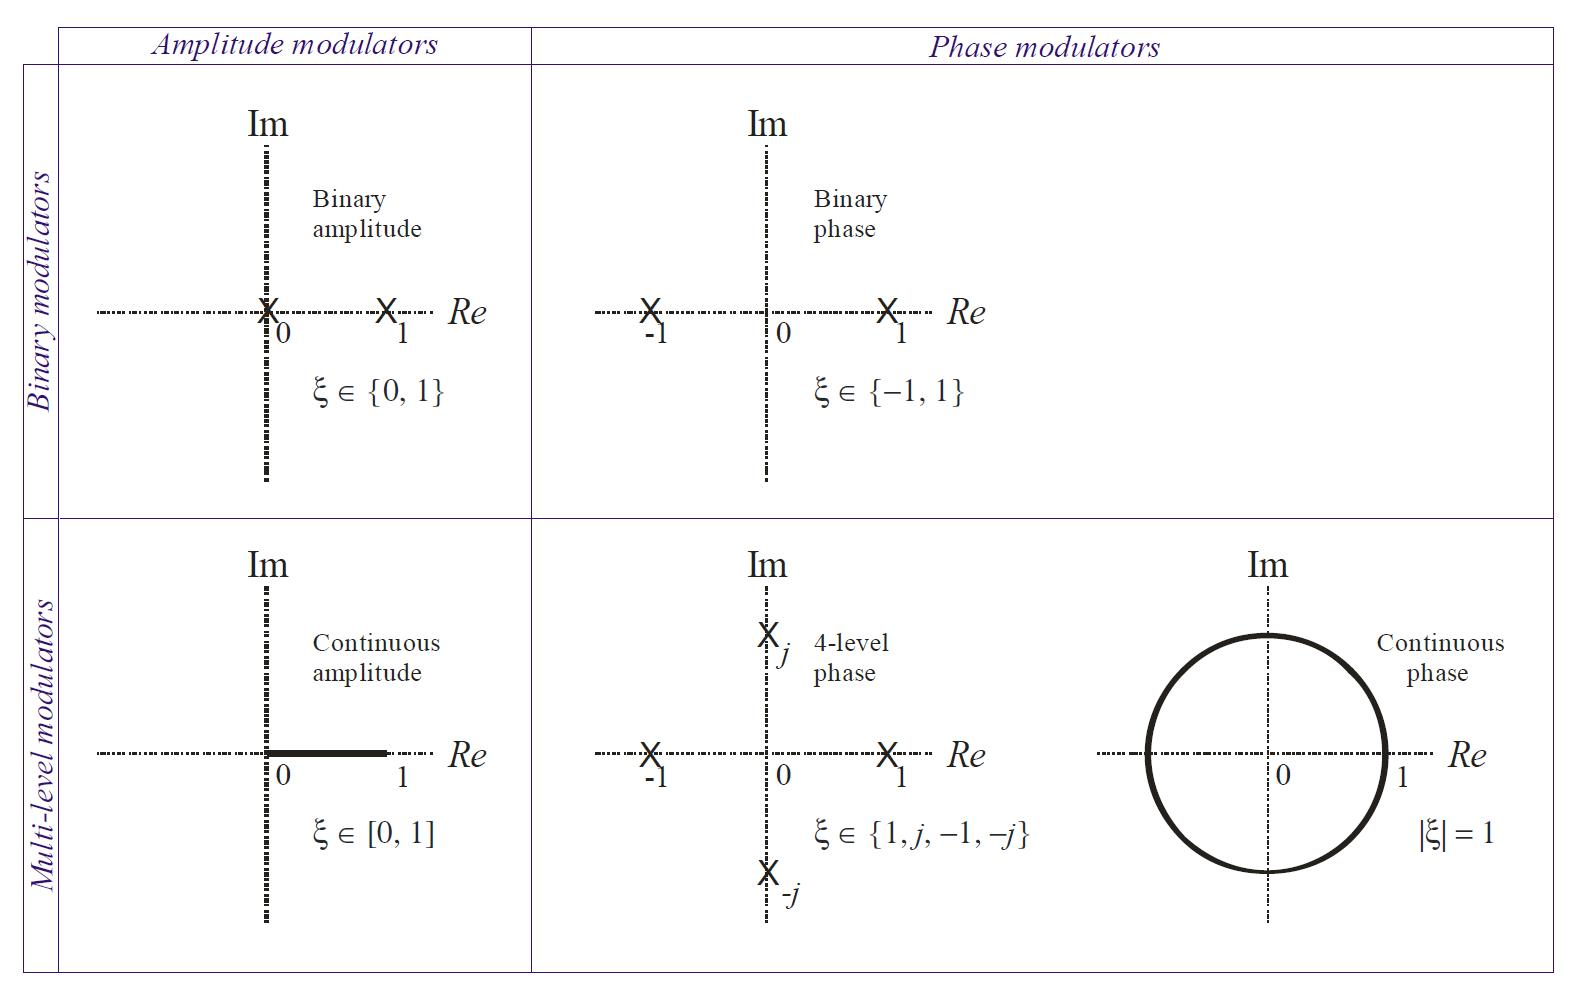
\includegraphics[width=0.9\textwidth]{modulation_loci.jpg}
  \caption{Modulation loci in the complex plane \cite{Cable2006}} \label{fig:modulation_loci}
\end{figure}

The four modulation schemes are \cite{Cable2006}:
\begin{itemize}
  \item \textbf{Multi-level Amplitude} modulators can modulate each pixel from zero transmission (0) to full transmission (1), either continuously or in discrete steps. (e.g. nematic liquid crystal display \cite{Schadt1971}, found for example in laptops and many conventional video projectors)
  \item \textbf{Binary Amplitude} modulators can switch each pixel to zero transmission (0) or full transmission (1), but nothing in between. (e.g. deformable mirror device \cite{Pape1983}, ferroelectric liquid crystal display \cite{Johnson1993}, both used in high-end video projectors)
  \item \textbf{Multi-level Phase} modulators can modulate the phase shift imparted by each pixel from 0 to 2$\pi$ radians, either continuously or in discrete steps. (e.g. Nematic liquid crystal devices \cite{Lee2004})
  \item \textbf{Binary Phase} modulators can switch each pixel for a phase shift of either 0 or $\pi$ radians. (e.g. Ferroelectric liquid crystal displays \cite{Broomfield1992})
\end{itemize}

Among the four modulation schemes, phase modulations are of higher interests, because amplitude modulations, either multi-level or binary, blocks light at the spatial light modulator (SLM), causing waste of energy, leading to poorer energy efficiency. And also, amplitude modulations always have a zero-order (forming a central bright spot), because the average amplitude is always between 0 and 1; on contrary, phase modulation can suppress the zero-order by forcing the hologram to have zero average, because the average of phase hologram can lie on 0 if well-designed.

The most common phase modulators are still only providing binary phase modulation, as the binary phase modulation is purely real (as it's only switching between $0^\circ$ and $180^\circ$), the complex conjugate $A^*(x,y)$ is the same as $A(x,y)$:
\begin{equation} \label{eq:AequalsAstar}
  A^*(x,y) = A(x,y)
\end{equation}
because the Fourier transform of $A^*(x,y)$ is the same as the Fourier transform of $A(x,y)$
\begin{equation} \label{eq:AAstar}
  E(-\alpha, -\beta)=\mathcal{F}[A^*(x,y)]=\mathcal{F}[A(x,y)]=E(\alpha, \beta)
\end{equation}
So there is no distinction between the desired image and its $180^\circ$ rotation in the replay field, causing a symmetrical conjugate image rotated $180^\circ$ from the target image. The simplest workaround for this issue is to use only half of the reconstruction field, and the computation of CGH for binary SLM will naturally need binary quantisation. Although few multi-level phase modulators are available, their bit depth is still limited (e.g. 4-bit 8-bit), so quantisation is still needed for the discrete levels, the effect of which is analysed in \cite{Kadis2022}.

In summary, before the invention of a complex modulator, we need algorithms to generate phase only hologram, such process is called phase retrieval. There are currently many algorithms for this purpose, which are discussed in \cref{sec:Naive algorithm} - \cref{sec:One Step Phase Retrieval (OSPR) Algorithm}.


\subsection{Naive Algorithm}\label{sec:Naive algorithm}
The naive algorithm to get a phase hologram is by directly using the phase of the reverse propagation from the target field to the hologram plane (e.g. for Fraunhofer propagation, the hologram is simply the inverse Fourier transform $\mathcal{F} ^{-1}$ of the target image), while discarding the amplitude component. The pseudocode of naive algorithm is shown in \cref{alg:Naive algorithm} below:
\begin{algorithm}[H]
  \caption{Naive algorithm}\label{alg:Naive algorithm}
  \textbf{Input:} Target field $T$, Propagation function $\mathcal{P}$ (e.g. Fresnel or Fraunhofer propagation)\\
  \textbf{Output:} Phase hologram $H$ and its reconstruction $R$
  \begin{algorithmic}
    \State $H \gets \angle\{\mathcal{P}^{-1}[T]\}$
    \State $R \gets \vert \mathcal{P}[e^{jH}] \vert$
  \end{algorithmic}
\end{algorithm}
where $j = \sqrt{-1} $. Naive algorithm (as described in \cref{alg:Naive algorithm}) was then implemented in MATLAB and the output results are shown in \cref{fig:Naive algorithm output} below:

\begin{figure}[H]
  \centering
  \begin{subfigure}[t]{0.3\textwidth}
    \centering
    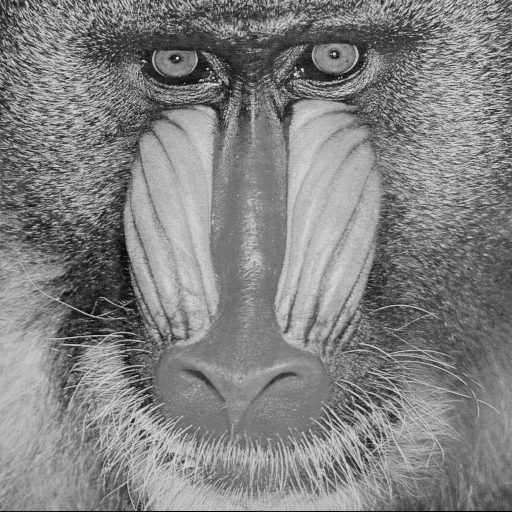
\includegraphics[width=\textwidth]{mandrill.png}
    \caption{Target field ($T$)}
  \end{subfigure}
  \hfill
  \begin{subfigure}[t]{0.3\textwidth}
    \centering
    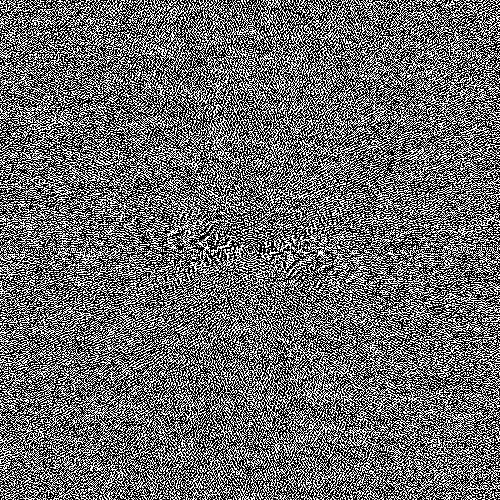
\includegraphics[width=\textwidth]{Naive_output_holo.png}
    \caption{Hologram ($H$)}
    \label{fig:Naive_output_holo}
  \end{subfigure}
  \hfill
  \begin{subfigure}[t]{0.3\textwidth}
    \centering
    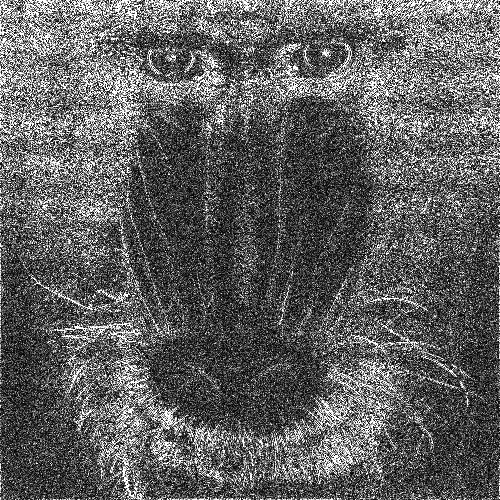
\includegraphics[width=\textwidth]{Naive_output_recon.png}
    \caption{Reconstruction ($R$)}
    \label{fig:Naive_output_recon}
  \end{subfigure}
  \caption{Naive algorithm output}
  \label{fig:Naive algorithm output}
\end{figure}

As shown in the simulation result, the reconstruction (\cref{fig:Naive_output_recon}) is very far from the desired target image. It has shown that, discarding amplitude introduces a significant loss of information.

Moreover, in order to display the hologram on a binary phase modulator or multi level phase modulator with limited bit-depth, the phase needs to be quantised again, introducing additional quantisation error.


\subsection{Direct Binary Search (DBS) Algorithm}\label{sec:Direct Binary Search (DBS) Algorithm}
Direct Binary Search (DBS) algorithm \cite{Seldowitz1987} is specifically designed for binary phase modulators, it generates the hologram by randomly flipping each pixel in the SLM between binary states, one by one for many times in order to minimise the difference between its reconstruction $R$ and the target image $T$. The detailed algorithm is described in \cref{alg:DBS algorithm} below:
\begin{algorithm}[H]
  \caption{Direct Binary Search (DBS) algorithm}\label{alg:DBS algorithm}
  \textbf{Input:} Target field $T$, Propagation function $\mathcal{P}$, Loss function $\mathcal{L}$, Number of iterations $N$ \\
  \textbf{Output:} Phase hologram $H$ and its reconstruction $R$
  \begin{algorithmic}
    \State{// Start with a random hologram with a size matching $T$}
    \State $H \gets$ Rand(Size($T$))
    \State $R \gets \vert \mathcal{P}[e^{jH}] \vert$
    \State $L \gets \mathcal{L} [R, T]$

    \For {$n$ = $1$ to $N$}
    \State{// Flip a random pixel in the hologram}
    \State $H_n \gets$ FlipRandomPixel($H$)\\
    \State{// Calculate the loss function for the new hologram}
    \State $R_n \gets \vert \mathcal{P}[e^{jH_n}] \vert$
    \State $L_n \gets \mathcal{L} [R_n, T]$\\
    \State{// Compare the new loss with the old one}
    \If {$L_n < L$}
    \State{// Accept the new hologram if loss is lower}
    \State $H \gets H_n$
    \State $R \gets R_n$
    \State $L \gets L_n$
    \EndIf
    \EndFor
  \end{algorithmic}
\end{algorithm}

\begin{figure}[H]
  \centering
  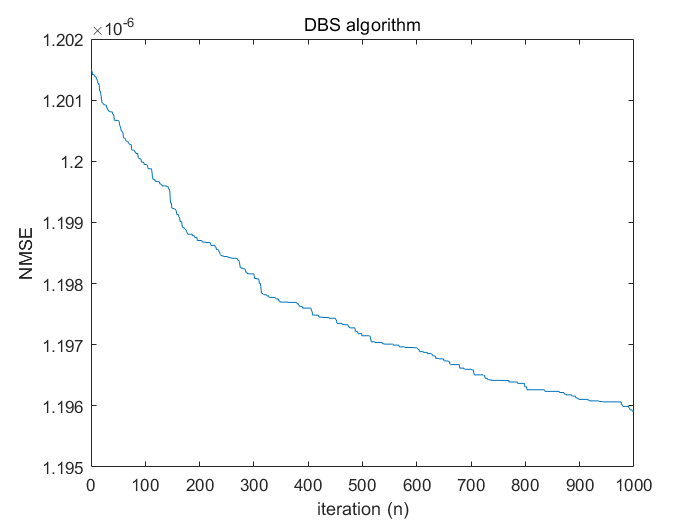
\includegraphics[width=0.7\textwidth]{DBS_NMSE_plot.png}
  \caption{DBS algorithm NMSE plot}
  \label{fig:DBS_NMSE_plot}
\end{figure}
DBS algorithm can sometimes find very accurate hologram if the run is lucky; however, it is extremely slow, because it takes numerous iterations (as shown in \cref{fig:DBS_NMSE_plot}, even 1000 iterations has not reached good convergence) and each iteration requires a Fourier transform which is computationally heavy. And also, as it only cares about local optimality at each iteration, it is a greedy algorithm that only follow the steepest descent route, which could easily get trapped in a local minimum where flipping any bit is not getting better reconstruction. Another consequence of the random nature is that the generated hologram will be different at each run, so the quality of the resulting reconstruction ($R$) will depend on how "lucky" each run is.


\subsection{Simulated Annealing (SA) Algorithm}\label{sec:Simulated Annealing (SA) Algorithm}
Simulated Annealing (SA) is an improvement on the DBS algorithm,
\cite{Kirkpatrick1983}. It adopts a probabilistic approach to avoid the steepest gradient descent. Its name derives from the fact that it approximates the recrystallisation process during metal annealing and is particularly well-suited to avoiding the trap of local minima \cite{Yang2009}. To implement this idea, we then need a function ($\mathcal{Q}$) to calculate the probability of the hologram ($H$), and a threshold $p_t$ to decide whether the probability is high enough for the according hologram to be accepted. The pseudocode for this algorithm is listed in \cref{alg:Simulated Annealing (SA) algorithm}.
\begin{algorithm}[H]
  \caption{Simulated Annealing (SA) algorithm}\label{alg:Simulated Annealing (SA) algorithm}
  \textbf{Input:} Target field $T$, Propagation function $\mathcal{P}$, Loss function $\mathcal{L}$, Number of iterations $N$, Probability function $\mathcal{Q}$ (e.g. Boltzmann Distribution), Probability threshold $p_t$ \\
  \textbf{Output:} Phase hologram $H$ and its reconstruction $R$
  \begin{algorithmic}
    \State{// Start with a random hologram with a size matching $T$}
    \State $H \gets$ Rand(Size($T$))
    \State $R \gets \vert \mathcal{P}[e^{jH}] \vert$
    \State $L \gets \mathcal{L} [R_0, T]$

    \For {$n$ = $1$ to $N$}
    \State{// Flip a random pixel in the hologram}
    \State $H_n \gets$ FlipRandomPixel($H$)\\
    \State{// Calculate the loss function for the new hologram}
    \State $R_n \gets \vert \mathcal{P}[e^{jH_n}] \vert$
    \State $L_n \gets \mathcal{L} [R_n, T]$\\
    \State{// Compare the new loss with the old one}
    \If {$L_n < L$}
    \State{// Accept the new hologram if loss is lower}
    \State $H \gets H_n$
    \State $R \gets R_n$
    \State $L \gets L_n$
    \Else
    \State{// Calculate the probability of the hologram}
    \State $p_n \gets \mathcal{Q}[H_n]$
    \If {$p_n > p_t$}
    \State{// Accept the new hologram if the probability exceeds the threshold}
    \State $H \gets H_n$
    \State $R \gets R_n$
    \State $L \gets L_n$
    \EndIf
    \EndIf
    \EndFor
  \end{algorithmic}
\end{algorithm}

\begin{figure}[H]
  \centering
  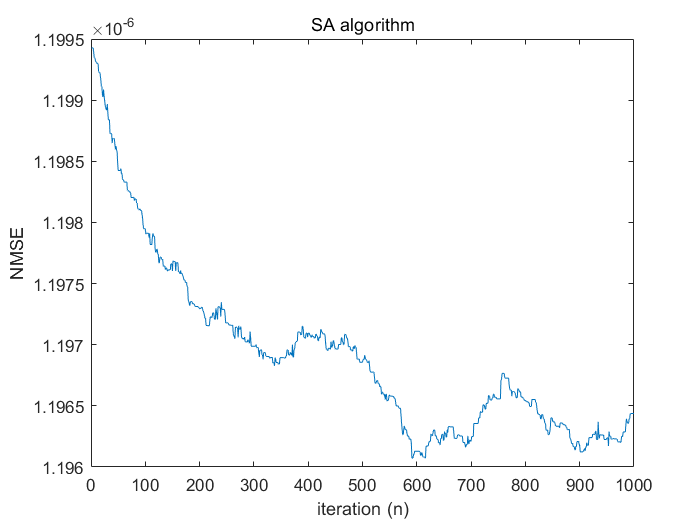
\includegraphics[width=0.7\textwidth]{SA_NMSE_plot.png}
  \caption{SA algorithm NMSE plot}
  \label{fig:SA_NMSE_plot}
\end{figure}
An implementation of SA algorithm with $p_t = 0.8$ was carried out, and the result is as shown in \cref{fig:SA_NMSE_plot}. It can be seen that, instead of monotonic decrease observed in \cref{fig:DBS_NMSE_plot} for DBS algorithm, the SA algorithm has occasional rises in NMSE, where the probability $p_n$ exceeds the threshold $p_t$.

\subsection{Gerchberg-Saxton (GS) algorithm}\label{sec:Gerchberg-Saxton (GS) Algorithm}
Gerchberg-Saxton (GS) algorithm functions that it iteratively determines the phase profile of the hologram required to reconstruct a target image; it loops between the hologram and the reconstruction plane, and applying constraints to each plane accordingly during each iteration \cite{Gerchberg1972}. GS algorithm is very easy to implement, its pseudocode is shown in \cref{alg:Gerchberg-Saxton (GS) Algorithm}.
\begin{algorithm}[H]
  \caption{Gerchberg-Saxton (GS) Algorithm}\label{alg:Gerchberg-Saxton (GS) Algorithm}
  \textbf{Input:} Target field $T$, Propagation function $\mathcal{P}$, Number of iterations $N$, Initial phase $\varPhi$ (e.g. random or zeros) \\
  \textbf{Output:} Phase hologram $H$ and its reconstruction $R$
  \begin{algorithmic}
    \State{// Initiate $E$ with amplitude $T$ and initial phase $\varPhi$}
    \State $E \gets T * e^{j\varPhi}$
    \For {$n$ = $1$ to $N$}
    \State{// Compute the hologram plane}
    \State $A \gets \mathcal{P}^{-1}[E]$
    \State{// Apply the phase-only constraint at the hologram plane}
    \State $A \gets e^{j\angle A}$\\
    \State{// Compute the propagation for the new hologram}
    \State $E \gets \mathcal{P}[A]$
    \State{// Apply the target field amplitude constraint at the hologram plane}
    \State $E \gets T * e^{j\angle E}$
    \EndFor
    \State $H \gets \angle A$
    \State $R \gets \vert \mathcal{P}[A] \vert$
  \end{algorithmic}
\end{algorithm}

The GS algorithm (described in \cref{alg:Gerchberg-Saxton (GS) Algorithm}) was implemented in MATLAB and the output results are shown in \cref{fig:GS algorithm output} below:

\begin{figure}[H]
  \centering
  \begin{subfigure}[t]{0.3\textwidth}
    \centering
    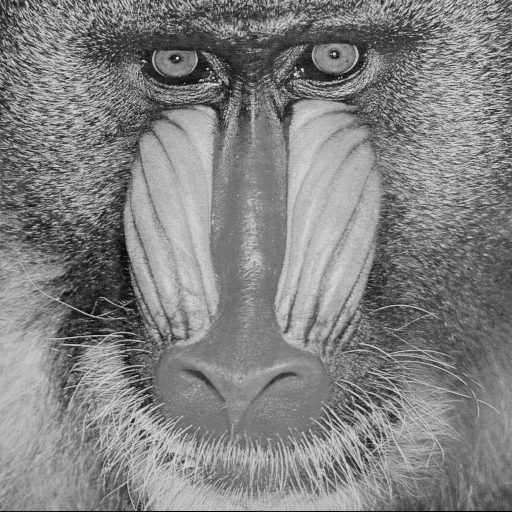
\includegraphics[width=\textwidth]{mandrill.png}
    \caption{Target field ($T$)}
  \end{subfigure}
  \hfill
  \begin{subfigure}[t]{0.3\textwidth}
    \centering
    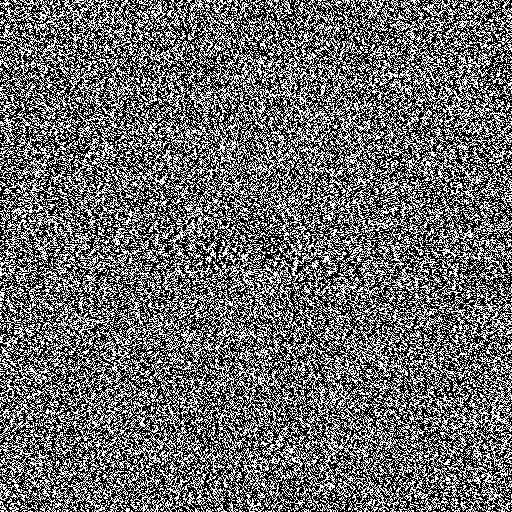
\includegraphics[width=\textwidth]{GS_holo_i_30.png}
    \caption{Hologram ($H$)}
    \label{fig:GS_holo_i_30}
  \end{subfigure}
  \hfill
  \begin{subfigure}[t]{0.3\textwidth}
    \centering
    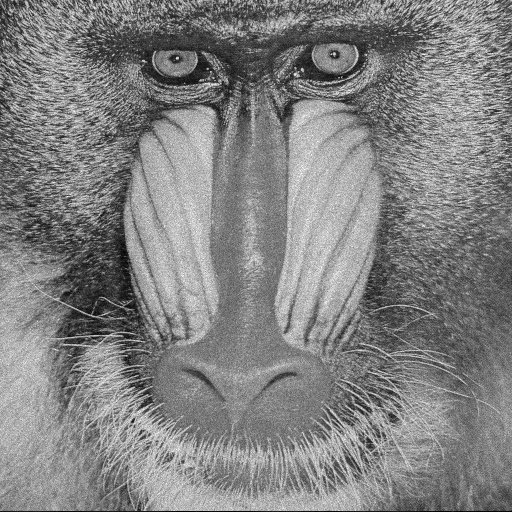
\includegraphics[width=\textwidth]{GS_recon_i_30.png}
    \caption{Reconstruction ($R$)}
    \label{fig:GS_recon_i_30}
  \end{subfigure}
  \caption{GS algorithm output for 30 iterations ($N = 30$)}
  \label{fig:GS algorithm output}
\end{figure}

It can be seen from \cref{fig:GS_recon_i_30} that, the reconstruction of the hologram after 30 iterations of GS algorithm reached a very good result. Then the quantitative analysis was carried out by measuring the normalised mean squared error (NMSE) as the iteration number ($n$) increments, the result is plotted in \cref{fig:GS_NMSE_plot}.

\begin{figure}[H]
  \centering
  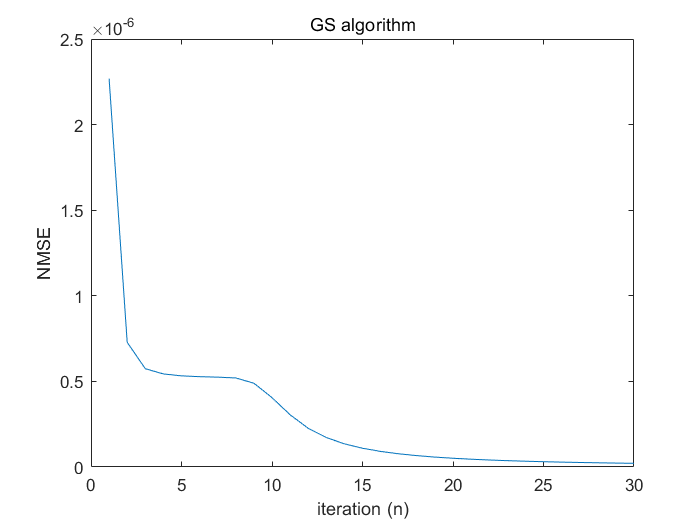
\includegraphics[width=0.7\textwidth]{GS_NMSE_plot.png}
  \caption{GS algorithm NMSE plot}
  \label{fig:GS_NMSE_plot}
\end{figure}

It can be seen from \cref{fig:GS_NMSE_plot} that GS algorithm converges quickly, providing very good result in tens of iterations. The major disadvantage of the GS algorithm is that it is more computationally expensive at every iteration, as it needs to compute both a forward and an inverse propagation function, causing the need for two Fourier transforms at each iteration. Nevertheless, the algorithm has very good performance over all.


\subsection{One-Step Phase Retrieval (OSPR) Algorithm}\label{sec:One Step Phase Retrieval (OSPR) Algorithm}
OSPR algorithm was first demonstrated by Buckley \cite{Buckley2006}. OSPR is a solution to high-quality hologram reconstruction that relies on time multiplexing of holograms, exploiting the response time of eye in order to reduce noise in the replay field \cite{Cable2006}. The random noises are averaged by the eye, while the target image stays, hence the average noise is reduced. The perceived noise is lessened by the temporal average detected by the eye, rather than computational optimisation of the hologram \cite{Cable2006}.
\begin{algorithm}[H]
  \caption{One-Step Phase Retrieval (OSPR) algorithm}\label{alg:One Step Phase Retrieval (OSPR) Algorithm}
  \textbf{Input:} Target field $T$, Propagation function $\mathcal{P}$, Number of sub-frames $S$ \\
  \textbf{Output:} List of phase holograms $H[1\ldots S]$
  \begin{algorithmic}
    \State // Compute a list of hologram sub-frames based on different additive random phase
    \For {$s$ = $1$ to $S$}
    \State $E \gets T * $ RandomPhase()
    \State $A \gets \mathcal{P}^{-1}[E]$
    \State $H[s] \gets \angle A$
    \EndFor\\
    \State // Then display the sub-frames on the phase modulator sequentially
    \State $s\gets 1$
    \While {True}
    \State Display(H[s])
    \State $s\gets s + 1$
    \If {$s > S$}
    \State $s\gets 1$
    \EndIf
    \EndWhile
  \end{algorithmic}
\end{algorithm}

The major advantage of the OSPR algorithm is that it is superfast, and also it can reduce the perceived speckle noise, providing a very good visual quality of holographic projection.


\subsection{Three-Dimensional (3D) CGH}\label{sec:Three-Dimensional (3D) CGH methods}
\cref{sec:Naive algorithm} - \cref{sec:One Step Phase Retrieval (OSPR) Algorithm} described several algorithms to generate a phase hologram for a single slice target field. Then the problem arises as how to generate a hologram for 3D target, and hence making full use of the major benefit of holography, which is true 3D reconstruction. There are several ways to achieve this.

\subsubsection{Multi-Layer Slicing}
The simplest method is to slice the 3D target into a set of layers, and then generate a set of phase holograms for each slice at its according distance ($z$) using Fresnel propagation model. Then the set of phase holograms are added up to form the final phase hologram, based on the principle of superposition.

\begin{figure}[H]
  \centering
  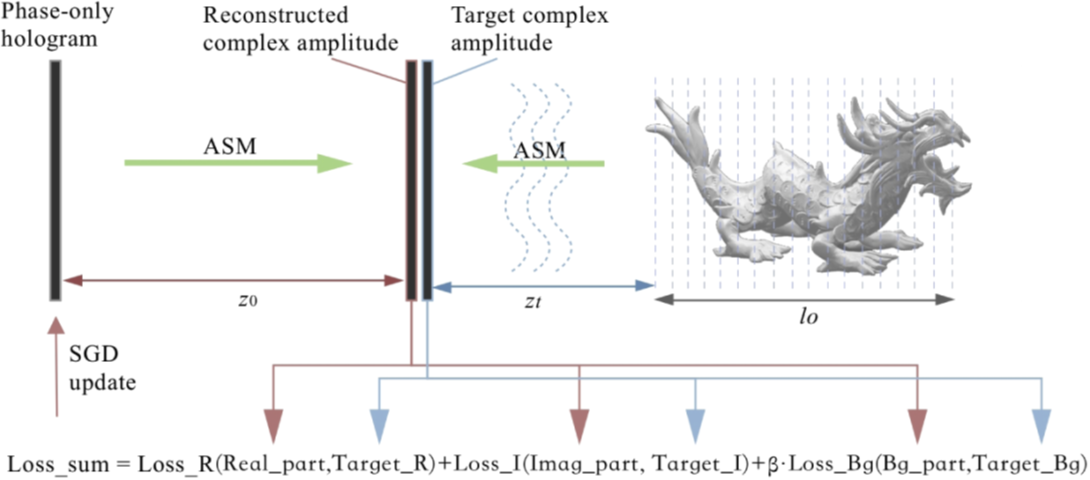
\includegraphics[width=0.9\textwidth]{intermediate_plane.png}
  \caption{Schematic diagram of the intermediate plane method \cite{Chen2021}}
  \label{fig:intermediate_plane}
\end{figure}

There is also an alternative solution, that is to propagate each slice of the 3D target into an intermediate plane, and then run the phase retrieval algorithms on the complex target field ($T$) with a loss function ($\mathcal{L} $), where needed, that accounts for both amplitude and phase components. The schematic of this method is shown in \cref{fig:intermediate_plane} \cite{Chen2021}.


\subsubsection{Point Cloud Method}
Point cloud method, as its name infers, divides a 3D target into a collection of points, each emitting a spherical wave, and then summed under the principle of superposition. The point cloud method is extremely computationally heavy and is very slow.



\newpage
\section{Numerical Optimisation Methods} \label{sec:Numerical Optimisation Methods}
In addition to the conventional CGH algorithms described in \cref{sec:cgh}, literature review has also found some recent work that compute CGH using numerical optimisation methods \cite{Zhang2017, Liu2020, Choi2021, Chen2021, Kadis2022}. This section is a review on what numerical optimisation is and how it works. And the implementation of optimisation of CGH is further discussed in \cref{sec:Numerical Optimisation of Phase-Only CGH}.

Numerical optimisation methods aim to find an optimal solution which minimise an objective function numerically. They begin with an initial guess of the optimal solution ($\textbf{x}_{0}$) and then, after iterations, generate a sequence of gradually improved estimates until they reach a solution \cite{Nocedal2006}. If we have $\textbf{x}$ as the vector of variables, and denote $f(\textbf{x})$ as the objective function, which is a function of $x$ we want to minimise, any unconstrained optimisation problem can be written as
\begin{equation}
  \underset{\textbf{x}\in R^n}{\text{minimise}}\quad f(\textbf{x})
  \label{eq:minimise_F}
\end{equation}

Numerical optimisation then calculate the optimal solution $\textbf{x}^*$ iteratively, the iteration is given by
\begin{equation}
  \textbf{x}_{k+1} = \textbf{x}_k+\alpha_k \textbf{p}_k
  \label{eq:optimisation_iteration}
\end{equation}
where the positive scalar $\alpha_k$ is called step length, or sometimes may be referred as `learning rate' in some context especially when related to machine learning, and the vector $\textbf{p}_k$ is the search direction, which usually takes the form of
\begin{equation}
  \textbf{p}_k = -\textbf{B}_k^{-1} \nabla f_{k} \label{eq:general-descent-direction}
\end{equation}
where $\textbf{B}_k$ is a nonsingular matrix that varies for different optimisation methods. The gradient $\nabla f_k$, if unable to evaluate directly, can be approximated by
\begin{align}
  \nabla f_k         & \approx \frac{f_{k+1}-f_{k}}{\textbf{x}_{k+1}-\textbf{x}_{k}} \nonumber \\
  \text{where}\  f_k & \ \text{denotes}\  f(\textbf{x}_k)
\end{align}

The strategy used to determine $\textbf{p}_k$ distinguishes one algorithm from another. Most methods make use of the values of $f$, $\nabla f$ and $\nabla^2 f$, and some methods even make use of the accumulated historical values of those derivatives, which are further discussed in \cref{sec:GD} - \cref{sec:L-BFGS}.

\subsection{Gradient Descent}\label{sec:GD}
Gradient descent (GD) is a first-order optimisation method, it finds a local minimum by following the negative of the gradient (i.e. the steepest descent direction). The $\textbf{B}_k$ (in \cref{eq:general-descent-direction}) for gradient descent simply takes the value of $\textbf{I}$, which is the identity matrix. And the search direction becomes:
\begin{equation}
  \textbf{p}_k = -\nabla f_k
\end{equation}
The steepest descent method is very intuitive: among all possible directions to move away from $\textbf{x}_{k}$, the steepest gradient direction is the one which $f$ decreases most rapidly. The advantage of this method is that it requires few computation and memory resource, because it only requires a computation of the first derivative, and it does not require any accumulation of historical gradients. However, it is a greedy method that only considers the current iteration without any global consideration, so it can be extremely slow on complicated problems. \cite{Nocedal2006}

To work around the disadvantage, a few variants have emerged, such as AdaGrad \cite{Duchi2011}, RMSProp \cite{Tieleman2012} and Adam \cite{Kingma2015} which combines the advantages of AdaGrad and RMSProp. It can be said to be an iconic variant of the gradient descent, often referred to as gradient descent with momentum. The name Adam is derived from adaptive moment estimation. Adam algorithm is based on adaptive estimates of lower-order moments \cite{Kingma2015}. Adam method computes individual adaptive learning rates for different parameters from estimates of first and second moments of the gradients \cite{Kingma2015}. Although some improvements are observed, it still does not fix entirely.


\subsection{Newton's Method}
Newton's method is a second-order optimisation method. Its search direction is derived from the second-order Taylor series approximation to $f(\textbf{x}_k+\textbf{p})$, which is
\begin{equation}
  f(\textbf{x}_k+\textbf{p}) \approx f_k + \textbf{p}^T \nabla f_k + \frac{1}{2}\textbf{p}^T \nabla^2 f_k \textbf{p} \stackrel{\text{def}}{=}m_k(\textbf{p})
\end{equation}
The Newton direction can then be obtained by finding the vector $\textbf{p}$ that minimises $m_k(\textbf{p})$. By setting the derivative of $m_k(\textbf{p})$ to zero, $\textbf{p}$ can be obtained as:
\begin{equation}
  \textbf{p}_k=-\nabla^2 f_k^{-1}\nabla f_k \label{eq:Newton-direction}
\end{equation}
By comparing \cref{eq:Newton-direction} to \cref{eq:general-descent-direction}, it can be seen that the Newton's method has a $\textbf{B}_k$ of $\nabla^2 f_k$. Unlike the gradient descent method, there is a "natural" step length of 1 associated with the Newton direction, so $\alpha_k = 1$ by default and is only adjusted when it does not produce a satisfactory reduction in the value of $f$.

The Newton direction is reliable when the difference between the true function $f(\textbf{x}_k+\textbf{p})$ and its quadratic model $m_k(\textbf{p})$ is not too large. Methods that use the Newton direction have a fast rate of local convergence, typically quadratic. After a neighbourhood of the solution is reached, convergence to high accuracy often occurs in just a few iterations. The main drawback of the Newton direction is the need for the Hessian $\nabla^2 f_k$. Explicit computation of this matrix of second derivatives can sometimes be a cumbersome, error-prone, and expensive process. \cite{Nocedal2006}



\subsection{Quasi-Newton Method: Broyden-Fletcher-Goldfarb-Shanno (BFGS)}\label{sec:BFGS}
Quasi-Newton method provides an attractive alternative to Newton's method, in that they do not require computation of the Hessian and yet still attain a super linear rate of convergence. In place of the true Hessian $\nabla^2 f_k$, they use an approximation $\textbf{H}_k \stackrel{\text{def}}{=} \textbf{B}_k^{-1}$, which is updated after each step to take account of the additional knowledge gained during the step. The updates make use of the fact that changes in the gradient provide information about the second derivative of $f$ along the search direction. The most popular quasi-Newton algorithm is the BFGS method, named for its discoverers Broyden, Fletcher, Goldfarb, and Shanno. \cite{Nocedal2006}

The process of the BFGS method is shown below:
\begin{align}
  denote   & \                       \left\{
  \begin{array}{ll}
    \textbf{H}_k & = \textbf{B}_k^{-1}          \\
    \textbf{p}_k & = -\textbf{H}_k \nabla f_{k}
  \end{array}
  \right.                                                                                                                                                                                                        \\
  Initiate & \ \textbf{H}_0     \leftarrow \frac{\textbf{y}_k^T\textbf{s}_k}{\textbf{y}_k^T\textbf{y}_k}\textbf{I}                                                           \label{eq:BFGS_initiate_H_0}        \\
  update   & \ \textbf{H}_{k+1}  = (\textbf{I} - \rho_k\textbf{s}_k\textbf{y}_k^T) \textbf{H}_{k} (\textbf{I} - \rho_k\textbf{y}_k\textbf{s}_k^T) +\rho_k\textbf{s}_k\textbf{s}_k^T \label{eq:BFGS_update_H_k+1} \\
  where    & \                        \left\{
  \begin{array}{ll}
    \textbf{s}_k & = \textbf{x}_{k+1} - \textbf{x}_{k}                               \\
    \textbf{y}_k & = \nabla f_{k+1} - \nabla f_{k}                                   \\
    \rho_k       & = \frac{1}{\textbf{y}_k^T\textbf{s}_k} \label{eq:BFGS_calc_rho_k}
  \end{array}
  \right.
\end{align}

The algorithm is robust, and its rate of convergence is super linear, which is fast enough for most practical purposes. Even though Newton's method converges more rapidly (that is, quadratically), its cost per iteration usually is higher, because of its need for second derivatives and solution of a linear system. The drawback is that, it is not directly applicable to large optimisation problems because $\textbf{H}_k$'s are usually dense, requiring large storage and computational requirements. \cite{Nocedal2006}



\subsection{Large Scale Quasi-Newton Method: Limited Memory BFGS (L-BFGS)}\label{sec:L-BFGS}
L-BFGS algorithm \cite{Liu1989} modifies the technique described in \cref{sec:BFGS} to obtain Hessian approximations that can be stored compactly in just a few vectors of length $n$, where $n$ is the number of unknowns in the problem. The main idea of this method is to use curvature information from only the most recent iterations to construct the Hessian approximation. Curvature information from earlier iterations, which is less likely to be relevant to the actual behaviour of the Hessian at the current iteration, is discarded in the interest of saving storage. \cite{Nocedal2006}

Denoting $\textbf{V}_k = \textbf{I} - \rho_k\textbf{y}_k\textbf{s}_k^T$, \cref{eq:BFGS_update_H_k+1} can be written as:
\begin{equation}
  \textbf{H}_{k+1} = \textbf{V}_k^T \textbf{H}_{k} \textbf{V}_k +\rho_k\textbf{s}_k\textbf{s}_k^T
\end{equation}

The inverse Hessian approximation $\textbf{H}_{k}$ will generally be dense, so that the cost of storing and manipulating it is prohibitive when the number of variables is large. To circumvent this problem, we store a modified version of $\textbf{H}_{k}$ implicitly, by storing a certain number (say, $m$) of the vector pairs $\{\textbf{s}_i, \textbf{y}_i\}$ used in the \cref{eq:BFGS_update_H_k+1} and \cref{eq:BFGS_calc_rho_k}. The product $\textbf{H}_{k} \nabla f_k$ can be obtained by performing a sequence of inner products and vector summations involving $\nabla f_k$ and the pairs $\{\textbf{s}_i, \textbf{y}_i\}$. After the new iterate is computed, the oldest vector pair in the set of pairs $\{\textbf{s}_i, \textbf{y}_i\}$ is replaced by the new pair $\{\textbf{s}_k, \textbf{y}_k\}$ obtained from the current step (\cref{eq:BFGS_calc_rho_k}). In this way, the set of vector pairs includes curvature information from the $m$ most recent iterations. Practical experience has shown that modest values of $m$ (between 3 and 20, say) often produce satisfactory results. We now describe the updating process in a little more detail. At iteration $k$, the current iterate is $\textbf{x}_k$ and the set of vector pairs is given by $\{\textbf{s}_i, \textbf{y}_i\}$ for $i=k-m,\ldots,k-1$. We first choose some initial Hessian approximation $\textbf{H}_{k}^0$ (in contrast to the standard BFGS iteration, this initial approximation is allowed to vary from iteration to iteration) and find by repeated application of \cref{eq:BFGS_update_H_k+1} that the L-BFGS approximation $\textbf{H}_{k}$ satisfies the following formula: \cite{Nocedal2006}

\begin{align}
  \textbf{H}_{k} =\  & (\textbf{V}_{k-1}^T \cdots \textbf{V}_{k-m}^T) \textbf{H}_{k}^0 (\textbf{V}_{k-m} \cdots \textbf{V}_{k-1})                                  \nonumber          \\
                     & + \rho_{k-m} (\textbf{V}_{k-1}^T \cdots \textbf{V}_{k-m+1}^T) \textbf{s}_{k-m} \textbf{s}_{k-m}^T (\textbf{V}_{k-m+1} \cdots \textbf{V}_{k-1}) \nonumber       \\
                     & + \rho_{k-m+1} (\textbf{V}_{k-1}^T \cdots \textbf{V}_{k-m+2}^T) \textbf{s}_{k-m+1} \textbf{s}_{k-m+1}^T (\textbf{V}_{k-m+2} \cdots \textbf{V}_{k-1}) \nonumber \\
                     & + \cdots \nonumber                                                                                                                                             \\
                     & + \rho_{k-1} \textbf{s}_{k-1} \textbf{s}_{k-1}^T
\end{align}

From this expression we can derive a recursive procedure (\cref{alg:L-BFGS}) to compute the product $\textbf{H}_{k} \nabla f_k$ efficiently.

\begin{algorithm}[H]
  \caption{L-BFGS two-loop recursion \cite{Nocedal2006}}\label{alg:L-BFGS}
  \begin{algorithmic}
    \State $\textbf{q} \gets \nabla f_k$
    \For{$i = k-1, k-2, ..., k-m$}
    \State $\alpha_i \gets \rho_i \textbf{s}_i^T \textbf{q}$
    \State $ \textbf{q} \gets \textbf{q} - \alpha_i\textbf{y}_i$
    \EndFor
    \State $\textbf{r}\gets \textbf{H}_k^0 \textbf{q}$
    \For{$i = k-m, k-m+1, ..., k-1$}
    \State $\beta \gets \rho_i \textbf{y}_i^T \textbf{r}$
    \State $ \textbf{r} \gets \textbf{r} +\textbf{s}_i (\alpha_i-\beta)$
    \EndFor
    \State Step with $\textbf{p}_k \gets -\textbf{H}_k \nabla f_{k} = -\textbf{r}$
  \end{algorithmic}
\end{algorithm}

Apart from being inexpensive, L-BFGS has the advantage that the multiplication by the initial matrix $\textbf{H}_k^0$ is isolated from the rest of the computations, allowing this matrix to be chosen freely and to vary between iterations. A method for choosing $\textbf{H}_k^0$ that has proved effective in practice is to use the same as BFGS as stated in \cref{eq:BFGS_initiate_H_0}. \cite{Nocedal2006}

